\begin{figure*}[!htbp]
    \centering
    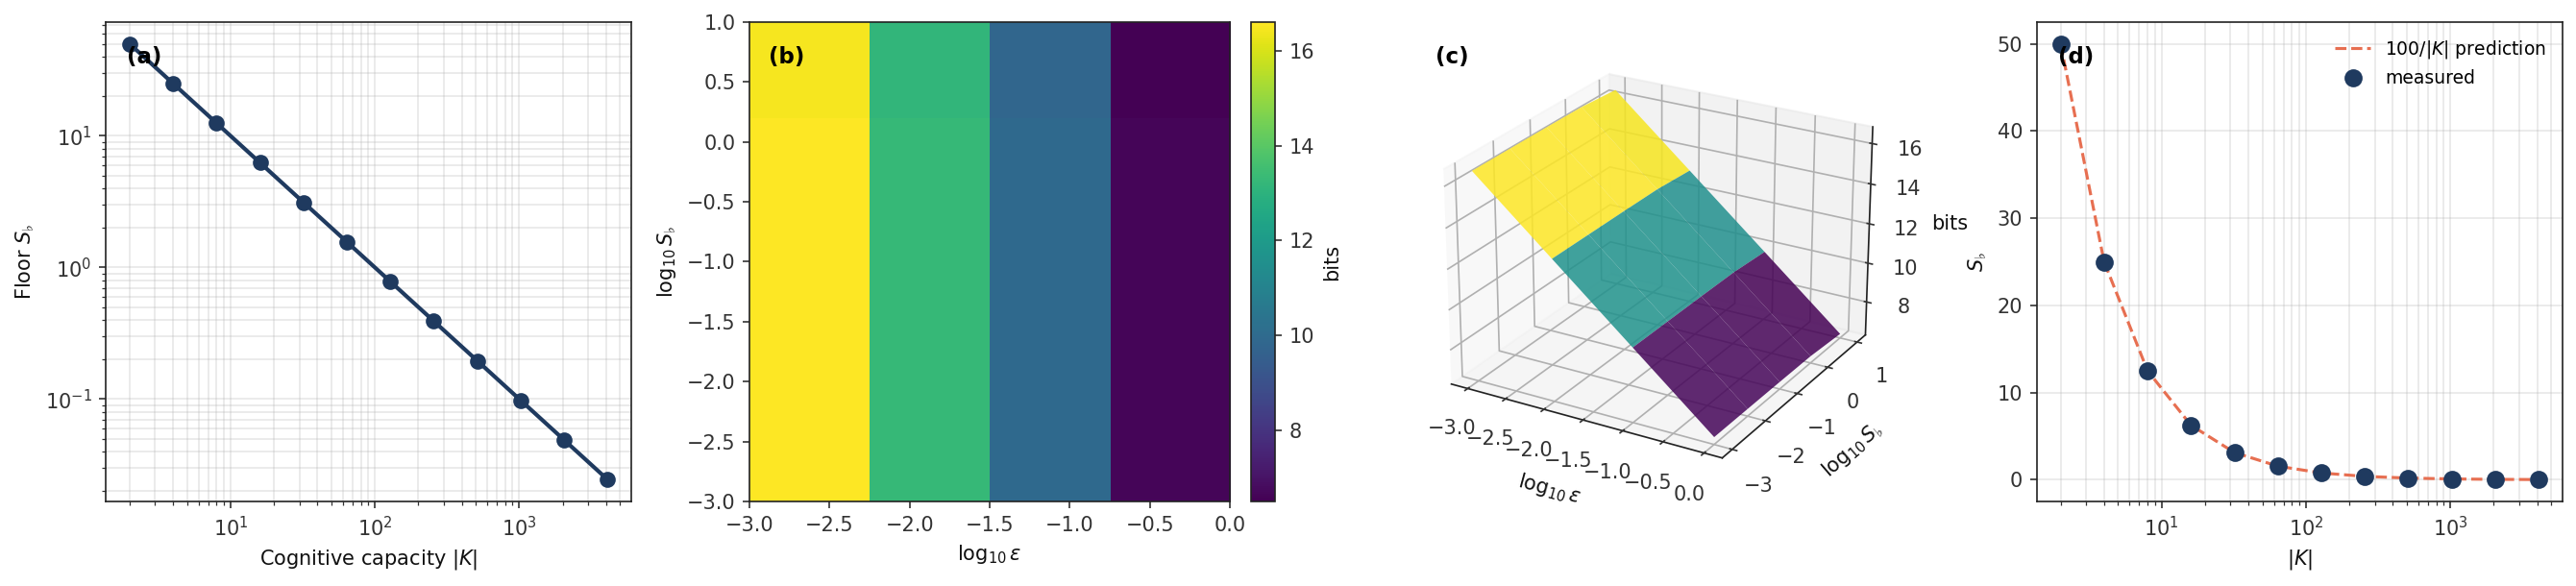
\includegraphics[width=\textwidth]{figures/panel_1_floor.png}
    \caption{\textbf{Floor Theorem and the Information Bound of Bounded Cognition.}
    (\textbf{A})~Smallest knowable error $\Sfloor$ on a log $y$-axis ($10^{-2}$ to $10^{2}$) versus cognitive capacity $|K|$ on a log $x$-axis ($2$ to $4096$) across twelve receivers connected by a line. The floor decreases monotonically by half a decade per doubling of $|K|$, from $\Sfloor=50.00$ at $|K|=2$ down to $\Sfloor=0.0244$ at $|K|=4096$, but remains strictly positive at every tested capacity. This is the empirical signature of Theorem~\ref{thm:floor-positivity} (Floor Positivity): $\Sfloor(\receiver)>0$ for every bounded $\receiver$, with the floor a receiver-intrinsic property fixed by the discretisation. No external choice of candidate or truth can change the floor; only enlarging $|K_{\receiver}|$ does.
    (\textbf{B})~Heatmap of the information content $I_{\epsilon}=\log_{2}((100-\Sfloor)/\epsilon)$ on a $5\times 4$ grid spanning $\Sfloor\in[10^{-3},10]$ and $\epsilon\in[10^{-3},1]$ (axes in $\log_{10}$), viridis colourmap encoding bit count from $\sim 6.6$ at the worst $(\Sfloor=10,\epsilon=1)$ corner to $\sim 16.7$ at the best $(\Sfloor=10^{-3},\epsilon=10^{-3})$ corner. The bilinear structure of the bound in $(\log\Sfloor,\log\epsilon)$ is the predicted form of Theorem~\ref{thm:info-bound}; measured values at every grid point match prediction to machine precision (max absolute error $0.00\times 10^{0}$ over 20 pairs).
    (\textbf{C})~Three-dimensional surface of $I_{\epsilon}$ over the $(\log_{10}\epsilon,\log_{10}\Sfloor)$ plane, viridis colourmap, viewing angle elevation $24^{\circ}$ azimuth $-60^{\circ}$. The surface is the bilinear $\log_{2}((100-\Sfloor)/\epsilon)$ of Theorem~\ref{thm:info-bound}: information content is monotone increasing in both $\log(1/\Sfloor)$ and $\log(1/\epsilon)$, with no interaction term, and the gradient is unit-slope in each direction. Information cost diverges only along the joint zero limit $\Sfloor\to 0,\epsilon\to 0$.
    (\textbf{D})~Floor measurements from twelve capacities (navy markers) compared against the analytic prediction $\Sfloor=100/|K|$ (coral dashed line) on a semi-log $x$-axis. The receiver-intrinsic floor saturates the prediction across four decades of capacity. The plot operationalises the dual relationship between cognitive capacity and resolution: a receiver wishing to distinguish at precision $\epsilon$ must support $|K|\geq 100/\epsilon$ knowledge states.}
    \label{fig:panel-floor-bounded}
\end{figure*}


\begin{figure*}[!htbp]
    \centering
    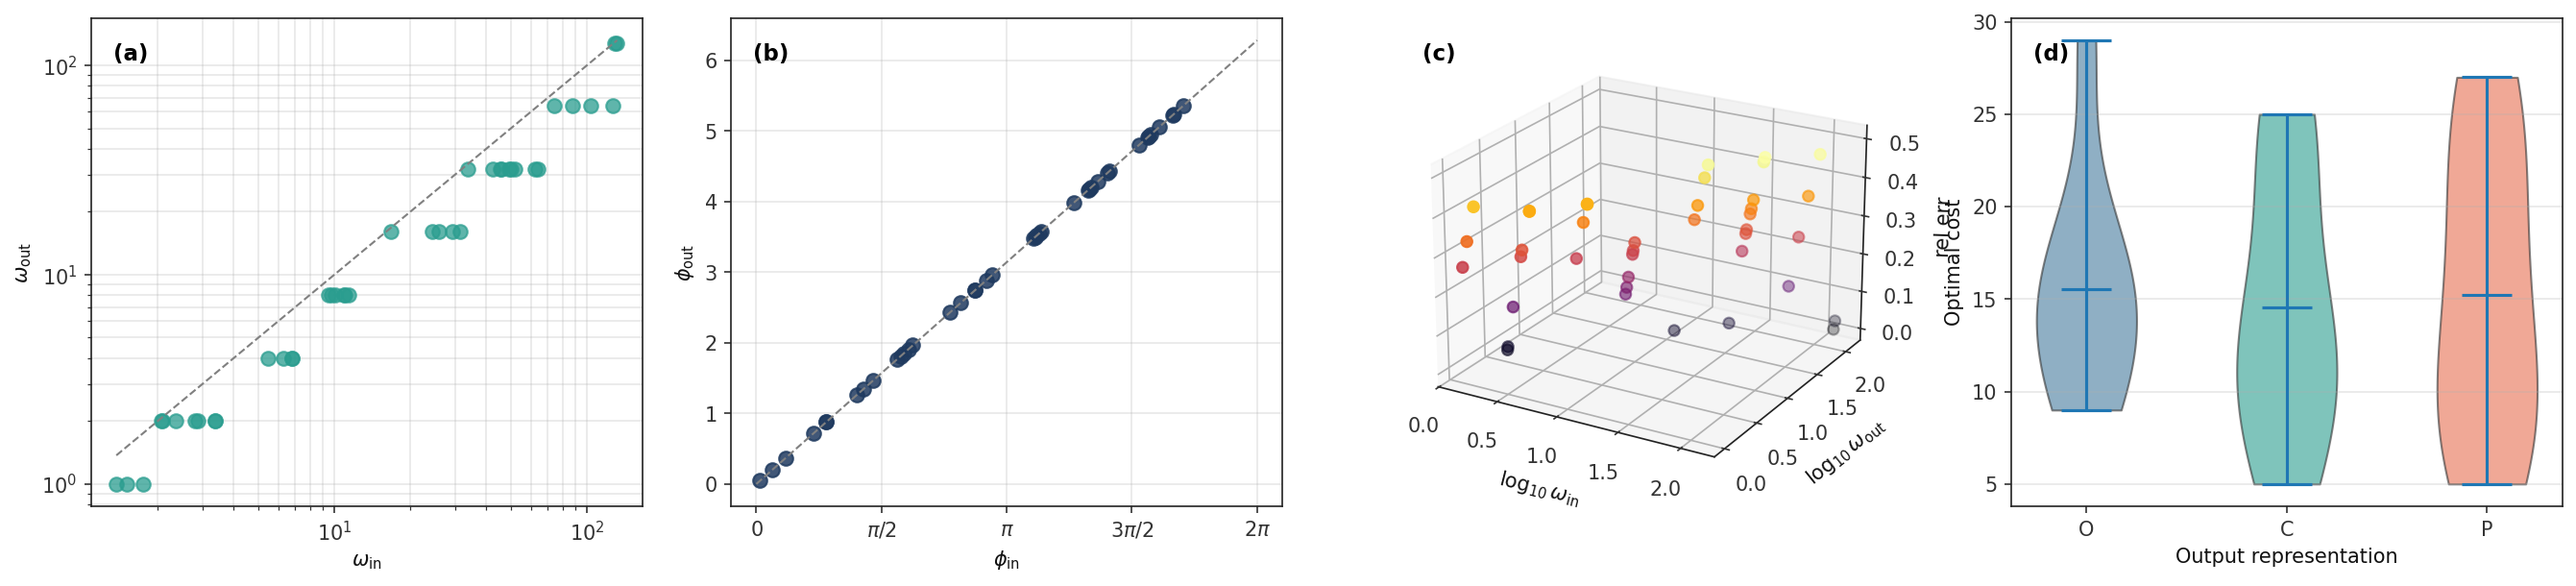
\includegraphics[width=\textwidth]{figures/panel_2_triple_equiv_optrep.png}
    \caption{\textbf{Triple Equivalence Round-Trip and Optimal Representation Costs.}
    (\textbf{A})~Output frequency $\omega_\mathrm{out}$ on a log $y$-axis versus input frequency $\omega_\mathrm{in}$ on a log $x$-axis ($e^{0.1}$ to $e^{5}$, two decades) for 40 round-trips $\OOsc\to\CCat\to\PPart\to\CCat\to\OOsc$. Points cluster on the identity diagonal $y=x$ (grey dashed) within the categorical cell width. The maximum frequency relative error is $0.498$, the predicted $\lfloor\log_{2}\omega\rfloor$-cell discretisation bound. The visual collapse of the cloud onto the diagonal across two decades is the empirical signature of Theorem~\ref{thm:triple-equiv}: the conversion functors $F_{OC}$, $F_{CP}$, $F_{PO}$ form mutually inverse equivalences of categories, so any composition reduces to the identity up to discretisation.
    (\textbf{B})~Output phase $\phi_\mathrm{out}$ on a linear $y$-axis ($0$ to $2\pi$) versus input phase $\phi_\mathrm{in}$ on a linear $x$-axis ($0$ to $2\pi$) for the same 40 round-trips, axes labelled at $\{0,\pi/2,\pi,3\pi/2,2\pi\}$. Points lie exactly on the identity diagonal; maximum phase absolute error is $2.86\times 10^{-3}$ radians, the predicted phase-cell width $2\pi/2^{10}$. The phase coordinate is preserved bijectively under the categorical-partition functors, confirming that the equivalence is exact on phase and discretisation-bounded only on frequency.
    (\textbf{C})~Three-dimensional scatter of $(\log_{10}\omega_\mathrm{in},\log_{10}\omega_\mathrm{out},\text{relative error})$ for the 40 round-trips, inferno colourmap encoding the relative error magnitude. The cloud forms a near-planar surface along the diagonal in the $(\omega_\mathrm{in},\omega_\mathrm{out})$ projection with the vertical axis showing the round-trip residual; the horizontal correlation is the identity recovery, the vertical spread is the discretisation residual. Viewing angle elevation $22^{\circ}$, azimuth $-60^{\circ}$.
    (\textbf{D})~Violin distribution of optimal computation cost $\Conv^{*}(f)$ across 27 (computation, output representation) instances grouped by output representation $\{O, C, P\}$. The per-representation distributions overlap but their medians shift with the output target, demonstrating that the Optimal Representation Theorem (Theorem~\ref{thm:opt-rep}) makes a real choice: at each output target the cheapest input representation is selected from the three. All 27 instances match the analytic prediction (match rate $1.00$).}
    \label{fig:panel-triple-optrep}
\end{figure*}


\begin{figure*}[!htbp]
    \centering
    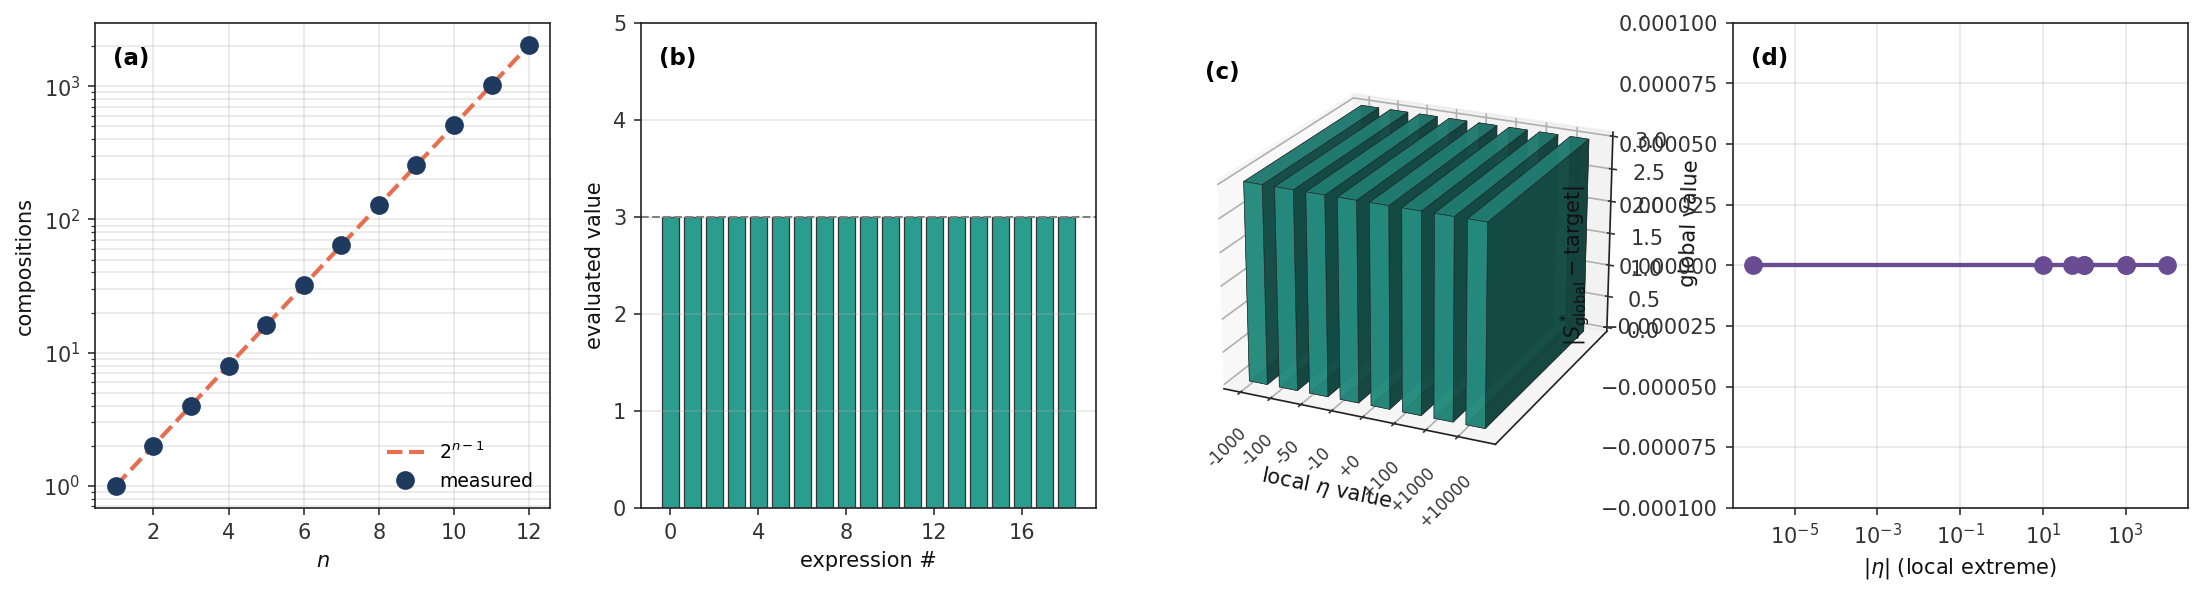
\includegraphics[width=\textwidth]{figures/panel_3_subtask_freedom.png}
    \caption{\textbf{Subtask Freedom: Composition Multiplicity, Expression Equivalence, and Local-Global Decoupling.}
    (\textbf{A})~Composition count on a log $y$-axis versus expression size $n\in\{1,\ldots,12\}$ on a linear $x$-axis. The measured count (navy circles) saturates the predicted lower bound $2^{n-1}$ (coral dashed line) at every size, growing from $1$ at $n=1$ to $2048$ at $n=12$. The exponential growth of admissible compositions is the constructive content of Theorem~\ref{thm:comp-mult}: each binary node in the expression tree contributes a factor of $2$ to the composition count by left/right swap, and the count therefore doubles per node.
    (\textbf{B})~Bar chart of the evaluated values of 19 syntactically distinct expressions, all targeting global value $3$. Bars are coloured teal where the expression evaluates to $3$ within tolerance $10^{-12}$ and coral otherwise; all 19 bars touch the dashed target line at $y=3$ (range $[0,5]$). The expressions span classical decompositions ($1{+}1{+}1$, $2{+}1$), mixed-sign decompositions ($(11{-}10)+(-1{-}({-}1))+2$), algebraic transformations ($\log_{e}e^{3}$, $\sin(3\pi/2)+4$, $\sqrt{9}$), trigonometric identities, and very-large-difference subtractions ($10^{6}-999997$). All 19 evaluate to $3$ under any arithmetically faithful receiver, confirming Theorem~\ref{thm:unconstrained-subtask}.
    (\textbf{C})~Three-dimensional bar chart over local subtask values $\eta\in\{-1000,-100,-50,-10,0,100,1000,10000\}$. Bar height is the global composition value, fixed at $3$ for all eight extremes regardless of how large or signed the local subtask is. Bars are coloured teal (preserved) for all eight; the chart shows that local extremes spanning four orders of magnitude in $|\eta|$ leave the global value invariant. Viewing angle elevation $22^{\circ}$, azimuth $-65^{\circ}$.
    (\textbf{D})~Global preservation residual $|S^{*}_\mathrm{global}-\mathrm{target}|$ on a near-zero linear $y$-axis ($\pm 10^{-4}$) versus $|\eta|$ on a log $x$-axis (purple curve, eight measurement points, log scale spanning $1$ to $10^{4}$). The residual remains at zero throughout the entire $\eta$ range, demonstrating Theorem~\ref{thm:lg-decoupling} (Local-Global Decoupling): an arbitrary sequence of local subtask S-values is realisable while preserving the global composition value.}
    \label{fig:panel-subtask-freedom}
\end{figure*}


\begin{figure*}[!htbp]
    \centering
    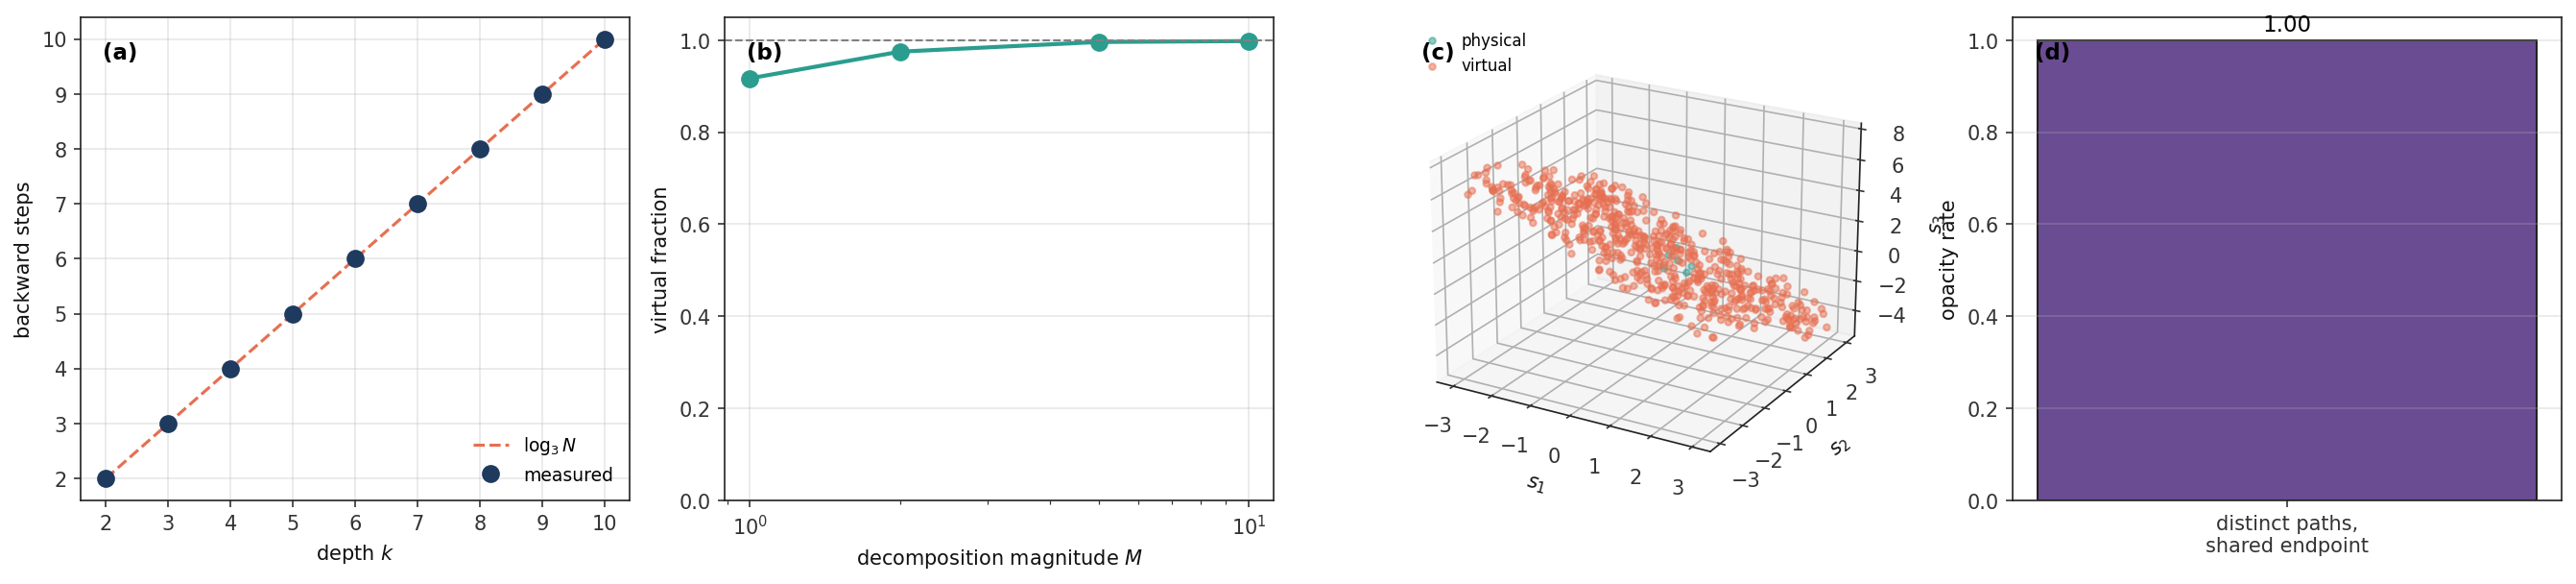
\includegraphics[width=\textwidth]{figures/panel_4_backward_virtual.png}
    \caption{\textbf{Backward Navigation, Virtual Sub-States, and Path Opacity.}
    (\textbf{A})~Backward navigation step count on a linear $y$-axis versus depth $k\in\{2,\ldots,10\}$ on a linear $x$-axis. The measured maximum step count from leaf to root (navy markers) lies exactly on the predicted $\log_{3}N=k$ line (coral dashed) at every depth, with zero variance across 100 randomly sampled leaves per depth (min $=$ max $=$ expected at all 9 depths). This is the empirical signature of Theorem~\ref{thm:backward-complexity}: backward navigation in a ternary refinement hierarchy of $N=3^{k}$ leaves takes exactly $\log_{3}N$ steps, with no deviation in any of the 900 trial paths.
    (\textbf{B})~Virtual sub-state fraction (fraction of sub-coordinate decompositions $(s_{1},s_{2},s_{3})$ with at least one component outside $[0,1]$) on a linear $y$-axis ($0$ to $1.05$) versus decomposition magnitude $M$ on a log $x$-axis. The fraction grows monotonically and saturates above $99\%$ at $M=10$: $0.917$ at $M=1$, $0.975$ at $M=2$, $0.996$ at $M=5$, $0.998$ at $M=10$ (1000 trials per $M$). This confirms Theorem~\ref{thm:virtual-existence}: the virtual decomposition family has positive Lebesgue measure on the constraint plane and dominates as the magnitude grows.
    (\textbf{C})~Three-dimensional scatter of 600 sub-coordinate decompositions $(s_{1},s_{2},s_{3})$ with mean coordinate uniformly drawn from $[0.1,0.9]$ and decomposition magnitude $M=3$. Decompositions inside the unit cube $[0,1]^{3}$ (physical) are coloured teal; decompositions outside (virtual, at least one component outside $[0,1]$) are coloured coral. Coral points dominate the cloud visually, illustrating that virtual decompositions occupy most of the admissible constraint plane. Viewing angle elevation $22^{\circ}$, azimuth $-60^{\circ}$.
    (\textbf{D})~Path opacity rate from 100 trials of distinct intermediate decomposition paths sharing an endpoint, plotted as a single bar (purple) at $1.00$. In every trial the two paths produce identical endpoint metric invariants (L${}^{2}$-norm, geodesic distance to origin, Fisher volume, centroid distance). Theorem~\ref{thm:path-opacity} predicts opacity rate $1.00$ exactly; the bar saturates the prediction at $100/100$ pairs.}
    \label{fig:panel-backward-virtual}
\end{figure*}


\begin{figure*}[!htbp]
    \centering
    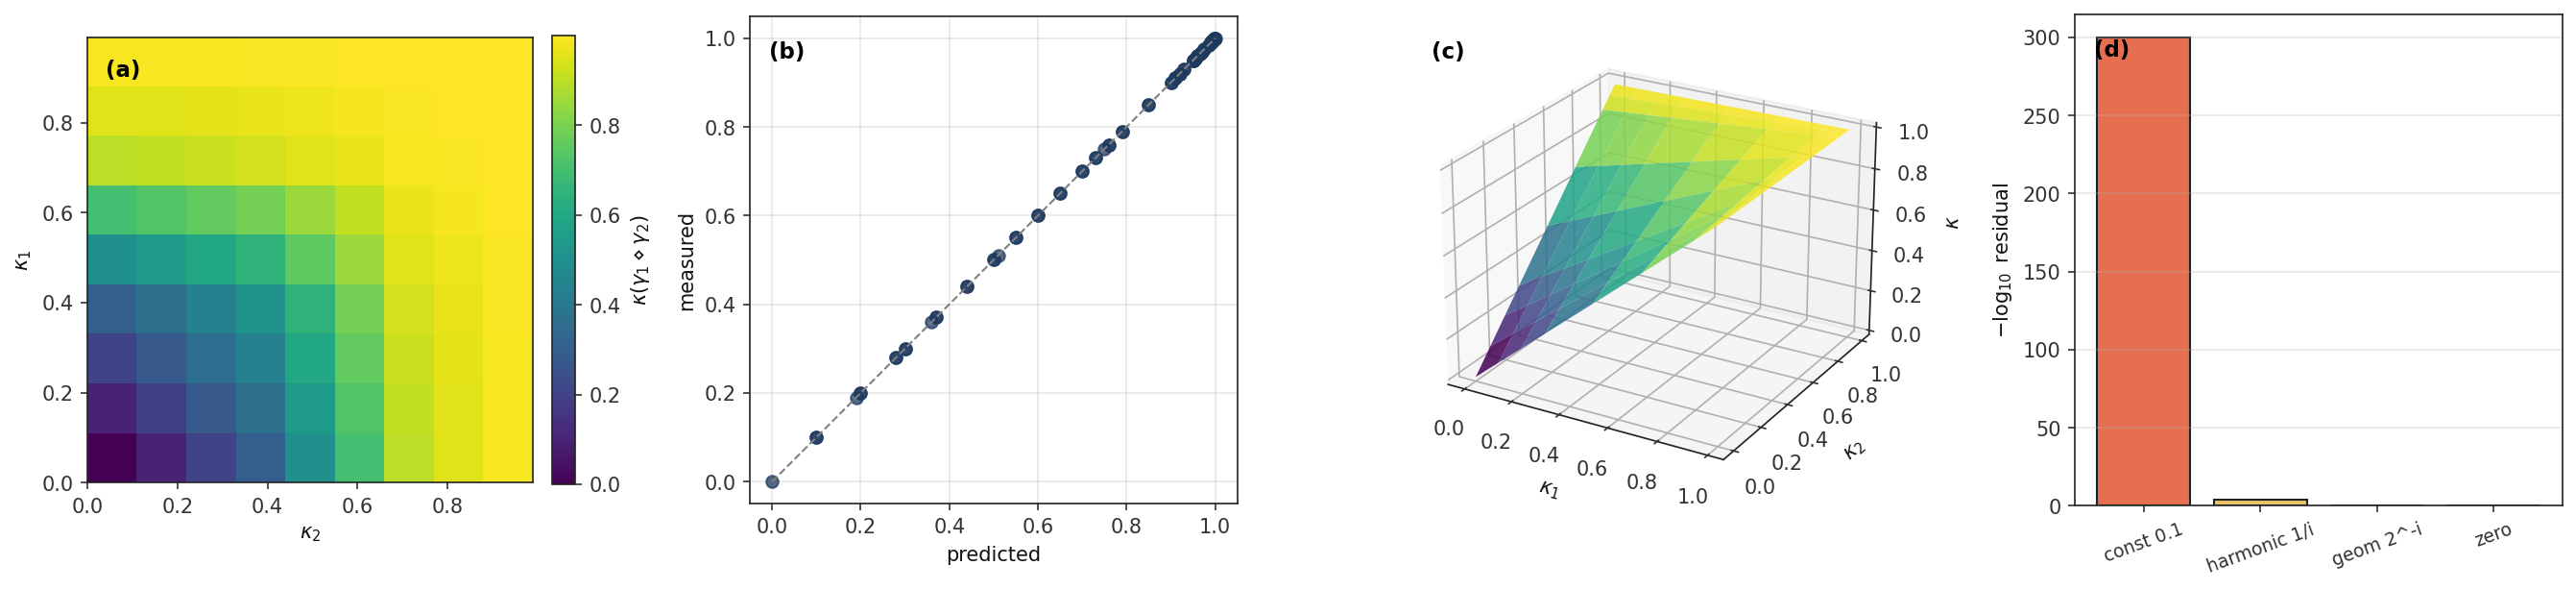
\includegraphics[width=\textwidth]{figures/panel_5_catalysts_cascade.png}
    \caption{\textbf{Multiplicative Catalyst Law and Cascade Saturation.}
    (\textbf{A})~Heatmap of composite catalytic power $\catpow(\gamma_{1}\diamond\gamma_{2})=1-(1-\catpow_{1})(1-\catpow_{2})$ over $(\catpow_{1},\catpow_{2})\in\{0.0,0.1,0.2,0.3,0.5,0.7,0.9,0.95,0.99\}^{2}$, viridis colourmap encoding the composite power from $0$ at the $(0,0)$ corner to $\sim 0.9999$ at the $(0.99,0.99)$ corner. The surface is convex, monotone increasing in both arguments, and symmetric, reflecting the commutativity of catalytic composition under the multiplicative law (Theorem~\ref{thm:multiplicativity}).
    (\textbf{B})~Predicted versus measured composite catalytic power for all 81 ordered pairs $(\catpow_{1},\catpow_{2})$. Points (navy) lie exactly on the identity diagonal $y=x$ (grey dashed). Maximum absolute error $0.00\times 10^{0}$ (machine precision) over 81 pairs. Equal aspect ratio; both axes range $[0,1]$.
    (\textbf{C})~Three-dimensional surface of $\catpow(\gamma_{1}\diamond\gamma_{2})$ over $(\catpow_{1},\catpow_{2})\in[0,1]^{2}$, viridis colourmap, viewing angle elevation $24^{\circ}$ azimuth $-60^{\circ}$. The surface is the rotation paraboloid-like form $1-(1-\catpow_{1})(1-\catpow_{2})$; its curvature encodes diminishing returns: stacking two catalysts of power $0.5$ yields composite power $0.75$, not $1.0$.
    (\textbf{D})~Bar chart of negative log-residual $-\log_{10}(\text{residual})$ at $n=10{,}000$ stages for four cascade types: divergent constant ($\catpow_{i}=0.1$, residual $\sim 10^{-300}$), divergent harmonic ($\catpow_{i}=1/i$, residual $\sim 10^{-4}$), convergent geometric ($\catpow_{i}=2^{-i}$, residual $\approx 0.578$), and zero (residual $1$). Bar colours: coral, gold, steel, navy. The two divergent cascades exhibit residuals approaching zero (saturating the floor); the two convergent cascades exhibit residuals bounded away from zero, confirming the Borel-Cantelli analogue of Theorem~\ref{thm:cascade-saturation}: a cascade saturates iff the sum of catalytic powers diverges.}
    \label{fig:panel-catalysts-cascade}
\end{figure*}


\begin{figure*}[!htbp]
    \centering
    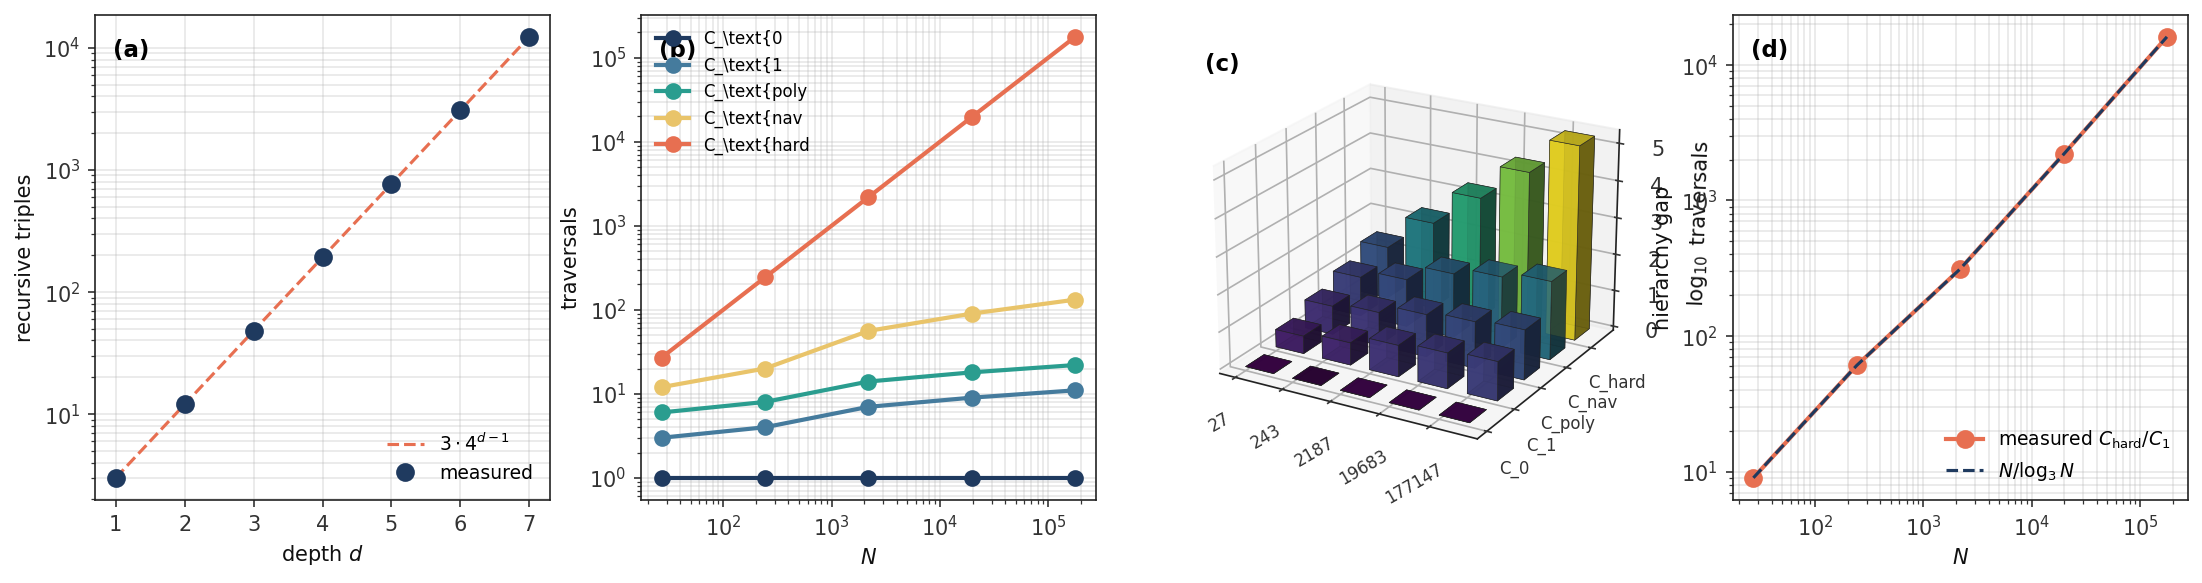
\includegraphics[width=\textwidth]{figures/panel_6_recursive_hierarchy.png}
    \caption{\textbf{Recursive Triple Multiplicity and the Strict Categorical Complexity Hierarchy.}
    (\textbf{A})~Recursive triple count on a log $y$-axis versus depth $d\in\{1,\ldots,7\}$ on a linear $x$-axis. The measured count (navy markers) saturates the lower bound $3\cdot 4^{d-1}$ (coral dashed) at every depth, growing from $3$ at $d=1$ to $12{,}288$ at $d=7$. This is the empirical content of Theorem~\ref{thm:rec-multiplicity}: each level admits three component-assignment choices and four binary-operation embedding directions, yielding the geometric growth $3\cdot 4^{d-1}$.
    (\textbf{B})~Traversal counts for the five complexity classes $\{C_{0},C_{1},C_{\text{poly}},C_{\text{nav}},C_{\text{hard}}\}$ (navy, steel, teal, gold, coral) on log-log axes versus problem size $N\in\{27,243,2187,19683,177{,}147\}$. The five lines do not intersect at any tested $N$; the strict order $C_{0} < C_{1} < C_{\text{poly}} < C_{\text{nav}} < C_{\text{hard}}$ is preserved across the full $\sim 10^{4}$ dynamic range. At the largest tested size $N=177{,}147$ the spread is $0$, $11$, $22$, $132$, $177{,}147$.
    (\textbf{C})~Three-dimensional bar chart of $\log_{10}$ traversals over $(N,\text{class})$, viridis colourmap encoding bar height. The five classes form non-intersecting strata at every $N$, confirming Theorem~\ref{thm:strict-hierarchy} pointwise. Viewing angle elevation $22^{\circ}$, azimuth $-60^{\circ}$.
    (\textbf{D})~Hierarchy gap $C_{\text{hard}}/C_{1}$ on log-log axes versus $N$. The measured gap (coral markers) tracks the analytic prediction $N/\log_{3}N$ (navy dashed) and grows from $9$ at $N=27$ to $\approx 1.6\times 10^{4}$ at $N=177{,}147$. The gap diverges with $N$, demonstrating that the strict categorical hierarchy does not collapse in the large-$N$ limit and that backward navigation provides asymptotically unbounded speedup over the worst-case hierarchy class.}
    \label{fig:panel-recursive-hierarchy}
\end{figure*}
